\documentclass{article}

% content/resources/templates/preamble.tex
\usepackage[margin=0.6in]{geometry}
\author{Milav Dabgar}
\usepackage{amsmath,amssymb,amsthm}
\usepackage{booktabs}
\usepackage{multirow}
\usepackage{xcolor}
\usepackage{tcolorbox}
\tcbuselibrary{breakable,skins}
\usepackage[colorlinks=true,linkcolor=blue]{hyperref}
\usepackage{titlesec}
\usepackage{enumitem}
\usepackage{tikz}
\usepackage{pgfplots}
\usepackage{circuitikz}
\usepackage[version=4]{mhchem}
\usepackage{longtable}
\usepackage{array}
\usepackage{float}
\usepackage{caption}
\usepackage{listings}

\lstset{
  basicstyle=\small\ttfamily,
  breaklines=true,
  breakatwhitespace=false,
  postbreak=\mbox{\textcolor{red}{$\hookrightarrow$}\space},
  float=false,
  numbers=left,
  numberstyle=\tiny\color{gray},
  numbersep=10pt,
  xleftmargin=2em,
  keywordstyle=\color{blue},
  commentstyle=\color{green!60!black},
  stringstyle=\color{purple},
  backgroundcolor=\color{gray!5},
  showstringspaces=false,
  tabsize=2,
  captionpos=b,
  keepspaces=true,
  columns=flexible
}

\pgfplotsset{compat=1.18}
\usetikzlibrary{shapes,arrows,positioning,calc,patterns,decorations.pathmorphing,decorations.markings,arrows.meta}

% Color scheme
\definecolor{headcolor}{RGB}{0,102,204}
\definecolor{keycolor}{RGB}{220,20,60}
\definecolor{solutioncolor}{RGB}{34,139,34}
\definecolor{mnemoniccolor}{RGB}{148,0,211}
\definecolor{codecolor}{RGB}{0,0,100}

% Spacing
\setlength{\parskip}{3pt}
\setlist[itemize]{nosep}
\setlist[enumerate]{nosep}

% Title formatting
\titleformat{\section}{\Large\bfseries\color{headcolor}}{\thesection}{1em}{}
\titleformat{\subsection}{\large\bfseries\color{headcolor}}{\thesubsection}{1em}{}

% Pandoc tightlist compatibility
\providecommand{\tightlist}{%
  \setlength{\itemsep}{0pt}\setlength{\parskip}{0pt}}

% Pandoc longtable compatibility
\newcounter{none}
\def\thenone{}


% content/resources/templates/english-boxes.tex

% Custom environments
\newtcolorbox{solutionbox}{
 breakable,
 enhanced,
 colback=solutioncolor!5!white,
 colframe=solutioncolor!75!black,
 fonttitle=\bfseries,
 title=Solution
}

\newtcolorbox{solutionboxnobreak}{
 colback=solutioncolor!5!white,
 colframe=solutioncolor!75!black,
 fonttitle=\bfseries,
 title=Solution
}

\newtcolorbox{keyformula}{
 breakable,
 enhanced,
 colback=keycolor!5!white,
 colframe=keycolor!75!black,
 fonttitle=\bfseries,
 title=Key Formula
}

\newtcolorbox{mnemonicboxenv}{
 breakable,
 enhanced,
 colback=mnemoniccolor!5!white,
 colframe=mnemoniccolor!75!black,
 fonttitle=\bfseries,
 title=Mnemonic
}

\newcommand{\mnemonicbox}[1]{%
  \begin{mnemonicboxenv}
    #1
  \end{mnemonicboxenv}
}


% Custom commands for GTU solutions
% This file defines semantic commands for consistent formatting

% Question command with automatic formatting
\newcommand{\question}[2]{%
  \section*{Question #1}%
  \textbf{#2}%
}

% OR question variant
\newcommand{\questionor}[2]{%
  \section*{Question #1 OR}%
  \textbf{#2}%
}

% Proper table environment with caption
\newenvironment{answertable}[1]{%
  \begin{table}[htbp]
  \centering
  \caption{#1}
}{%
  \end{table}
}

% Proper figure environment for diagrams
\newenvironment{answerdiagram}[1]{%
  \begin{figure}[htbp]
  \centering
  \caption{#1}
}{%
  \end{figure}
}

% Semantic markup for key terms
\newcommand{\keyword}[1]{\textbf{#1}}
\newcommand{\code}[1]{\texttt{#1}}
\newcommand{\classname}[1]{\texttt{#1}}
\newcommand{\methodname}[1]{\texttt{#1}}

% Proper quotation marks
\newcommand{\mnemonic}[1]{``#1''}


\title{Principles of Electronic Communication (4331104) - Winter 2023 Solution}
\date{January 20, 2023}

\begin{document}
\maketitle

\questionmarks{1}{a}{3}
\textbf{Classify Noise signal and explain thermal noise.}

\begin{solutionbox}
    \textbf{Classification of Noise Signals:}

    \begin{center}
    \begin{tabulary}{\linewidth}{L L L}
        \hline
        \textbf{Type of Noise} & \textbf{Source} & \textbf{Characteristics} \\
        \hline
        \textbf{External Noise} & Outside communication system & Atmospheric, Space, Industrial \\
        \textbf{Internal Noise} & Inside communication system & Thermal, Shot, Transit time, Flicker \\
        \hline
    \end{tabulary}
    \captionof{table}{Noise Classification}
    \end{center}

    \textbf{Thermal Noise:}
    \begin{itemize}
        \item \textbf{Definition}: Random motion of electrons in a conductor due to temperature. also known as Johnson-Nyquist noise.
        \item \textbf{Characteristics}: White noise with uniform power across frequency spectrum.
        \item \textbf{Formula}: $N = kTB$
        \begin{itemize}
            \item $k$: Boltzmann constant ($1.38 \times 10^{-23}$ J/K)
            \item $T$: Temperature in Kelvin
            \item $B$: Bandwidth in Hertz
        \end{itemize}
    \end{itemize}

    \begin{mnemonicbox}
    "TERM" - Temperature Excites Random Movements
    \end{mnemonicbox}
\end{solutionbox}

\questionmarks{1}{b}{4}
\textbf{Comparison between Pre-emphasis and De-emphasis technique.}

\begin{solutionbox}
    \textbf{Comparison of Pre-emphasis and De-emphasis:}

    \begin{center}
    \begin{tabulary}{\linewidth}{L L L}
        \hline
        \textbf{Parameter} & \textbf{Pre-emphasis} & \textbf{De-emphasis} \\
        \hline
        \textbf{Definition} & Boosting high-frequency components before transmission & Attenuating high-frequency components at receiver \\
        \textbf{Location} & Transmitter side & Receiver side \\
        \textbf{Purpose} & Improves SNR for high frequencies & Restores original signal frequency response \\
        \textbf{Circuit} & High-pass filter with RC circuit & Low-pass filter with RC circuit \\
        \textbf{Time Constant} & 75 $\mu$s (standard) & 75 $\mu$s (matches pre-emphasis) \\
        \hline
    \end{tabulary}
    \captionof{table}{Pre-emphasis vs De-emphasis}
    \end{center}

    \begin{center}
    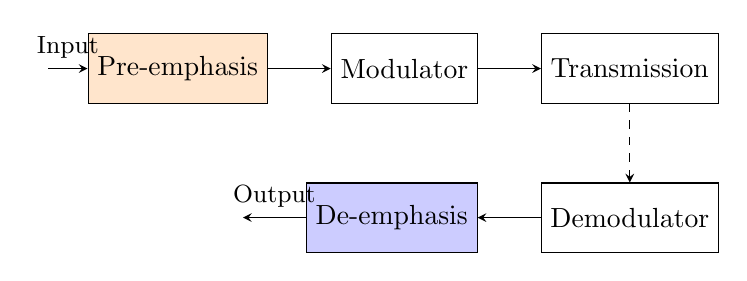
\begin{tikzpicture}[auto, node distance=1.5cm,
        block/.style={draw, rectangle, minimum height=2.5em, minimum width=3.5em, align=center, fill=white},
        >=stealth
    ]
        \node [coordinate] (input) {};
        \node [block, right=0.5cm of input, fill=orange!20] (pre) {Pre-emphasis};
        \node [block, right=0.8cm of pre] (mod) {Modulator};
        \node [block, right=0.8cm of mod] (tx) {Transmission};
        \node [block, below=1cm of tx] (demod) {Demodulator};
        \node [block, left=0.8cm of demod, fill=blue!20] (de) {De-emphasis};
        \node [coordinate, left=0.8cm of de] (out) {};

        \draw [->] (input) -- node[above, font=\small]{Input} (pre);
        \draw [->] (pre) -- (mod);
        \draw [->] (mod) -- (tx);
        \draw [->, dashed] (tx) -- (demod);
        \draw [->] (demod) -- (de);
        \draw [->] (de) -- node[above, font=\small]{Output} (out);
    \end{tikzpicture}
    \captionof{figure}{Pre-emphasis and De-emphasis in FM System}
    \end{center}

    \begin{mnemonicbox}
    "PUBTAR" - Pump Up Before Transmit, Pull Down After Receive
    \end{mnemonicbox}
\end{solutionbox}

\questionmarks{1}{c}{7}
\textbf{Derive mathematical expression of AM signal and with help of it explain frequency spectrum of AM signal.}

\begin{solutionbox}
    \textbf{Mathematical Expression Derivation:}

    1. Let the carrier signal be:
    \[ c(t) = A_c \cos(2\pi f_c t) \]
    2. Let the modulating signal be:
    \[ m(t) = A_m \cos(2\pi f_m t) \]
    3. The Amplitude Modulated signal $s(t)$ is given by:
    \[ s(t) = A_c[1 + \mu \frac{m(t)}{A_m}]\cos(2\pi f_c t) \]
       where $\mu = \frac{A_m}{A_c}$ is the modulation index.
    4. Substituting $m(t)$:
    \[ s(t) = A_c[1 + \mu \cos(2\pi f_m t)]\cos(2\pi f_c t) \]
    5. Expanding the expression:
    \[ s(t) = A_c \cos(2\pi f_c t) + \mu A_c \cos(2\pi f_m t)\cos(2\pi f_c t) \]
    6. Using trigonometric identity $\cos(A)\cos(B) = \frac{1}{2}[\cos(A+B) + \cos(A-B)]$:
    \[ s(t) = A_c \cos(2\pi f_c t) + \frac{\mu A_c}{2} [\cos(2\pi(f_c+f_m)t) + \cos(2\pi(f_c-f_m)t)] \]
    
    This is the mathematical expression of AM signal.

    \textbf{Frequency Spectrum:}
    
    \begin{center}
    \begin{tabulary}{\linewidth}{L L L}
        \hline
        \textbf{Component} & \textbf{Frequency} & \textbf{Amplitude} \\
        \hline
        Carrier & $f_c$ & $A_c$ \\
        Upper Sideband (USB) & $f_c + f_m$ & $\frac{\mu A_c}{2}$ \\
        Lower Sideband (LSB) & $f_c - f_m$ & $\frac{\mu A_c}{2}$ \\
        \hline
    \end{tabulary}
    \captionof{table}{AM Spectrum Components}
    \end{center}

    \begin{center}
    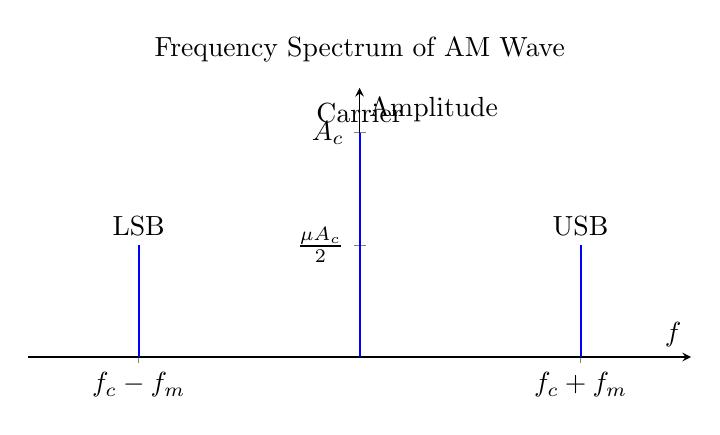
\begin{tikzpicture}
        \begin{axis}[
            width=10cm, height=5cm,
            axis lines=middle,
            xtick={-1,0,1}, 
            xticklabels={$f_c-f_m$, $f_c$, $f_c+f_m$},
            ytick={0, 0.5, 1},
            yticklabels={0, $\frac{\mu A_c}{2}$, $A_c$},
            ymin=0, ymax=1.2,
            xmin=-1.5, xmax=1.5,
            xlabel={$f$}, ylabel={Amplitude},
            title={Frequency Spectrum of AM Wave}
        ]
            \addplot[ycomb, mark=none, thick, blue] coordinates {
                (0, 1) (-1, 0.5) (1, 0.5)
            };
            \node[above] at (axis cs:0,1) {Carrier};
            \node[above] at (axis cs:-1,0.5) {LSB};
            \node[above] at (axis cs:1,0.5) {USB};
        \end{axis}
    \end{tikzpicture}
    \captionof{figure}{AM Frequency Spectrum}
    \end{center}

    \begin{mnemonicbox}
    "CSBT" - Carrier Standing Between Twins
    \end{mnemonicbox}
\end{solutionbox}

\questionmarks{1}{c}{7}
\textbf{Explain block diagram of Communication System.}

\begin{solutionbox}
    \textbf{Block Diagram of Communication System:}

    \begin{center}
    \begin{tikzpicture}[auto, node distance=2cm,
        block/.style={draw, rectangle, minimum height=3em, minimum width=4em, align=center, fill=white},
        noise/.style={draw, circle, fill=red!20},
        >=stealth
    ]
        \node [coordinate] (source) {};
        \node [block, right=0.5cm of source] (input) {Input Transducer};
        \node [block, right=1cm of input] (tx) {Transmitter};
        \node [block, right=1.5cm of tx] (rx) {Receiver};
        \node [block, right=1cm of rx] (output) {Output Transducer};
        \node [coordinate, right=0.5cm of output] (dest) {};
        
        % Channel
        \node [coordinate] (ch_in) at ($(tx.east)!0.5!(rx.west)$);
        \node [block, below=1.5cm of ch_in, minimum width=6em] (channel) {Channel / Medium};
        \node [noise, right=1cm of channel] (noise) {Noise};
        
        \draw [->] (source) -- node[above, font=\small]{Info} (input);
        \draw [->] (input) -- node[above, font=\small]{Elec. Signal} (tx);
        \draw [->] (tx) -| (channel);
        \draw [->] (channel) |- (rx);
        \draw [->] (rx) -- node[above, font=\small]{Original Info} (output);
        \draw [->] (output) -- (dest);
        \draw [->, dashed, red] (noise) -- (channel);

    \end{tikzpicture}
    \captionof{figure}{Elements of Communication System}
    \end{center}

    \textbf{Components and Functions:}

    \begin{center}
    \begin{tabulary}{\linewidth}{L L L}
        \hline
        \textbf{Block} & \textbf{Function} & \textbf{Example} \\
        \hline
        \textbf{Input Transducer} & Converts original information to electrical signal & Microphone, Camera \\
        \textbf{Transmitter} & Processes signal for efficient transmission (modulation, amplification) & Radio transmitter \\
        \textbf{Channel/Medium} & Path through which signal travels & Air, Fiber, Cable \\
        \textbf{Receiver} & Extracts original signal (amplification, filtering, demodulation) & Radio receiver \\
        \textbf{Output Transducer} & Converts electrical signal back to original form & Speaker, Display \\
        \textbf{Noise Source} & Unwanted signals that distort the information & Atmospheric, Thermal \\
        \hline
    \end{tabulary}
    \captionof{table}{System Components}
    \end{center}

    \begin{mnemonicbox}
    "ITCRO" - Input Transmits Through Channel, Receives Output
    \end{mnemonicbox}
\end{solutionbox}

\questionmarks{2}{a}{3}
\textbf{Discuss power distribution among sidebands and carrier in amplitude modulation.}

\begin{solutionbox}
    \textbf{Power Distribution in AM Signal:}

    Total power $P_t$ is the sum of carrier power $P_c$ and sideband power $P_{SB}$.

    \begin{center}
    \begin{tabulary}{\linewidth}{L L L}
        \hline
        \textbf{Component} & \textbf{Power Formula} & \textbf{Percentage ($m=1$)} \\
        \hline
        Carrier & $P_c = \frac{A_c^2}{2R}$ & 66.7\% \\
        Upper Sideband & $P_{USB} = \frac{P_c \mu^2}{4}$ & 16.65\% \\
        Lower Sideband & $P_{LSB} = \frac{P_c \mu^2}{4}$ & 16.65\% \\
        Total Power & $P_T = P_c(1 + \frac{\mu^2}{2})$ & 100\% \\
        \hline
    \end{tabulary}
    \captionof{table}{AM Power Distribution}
    \end{center}

    \begin{center}
    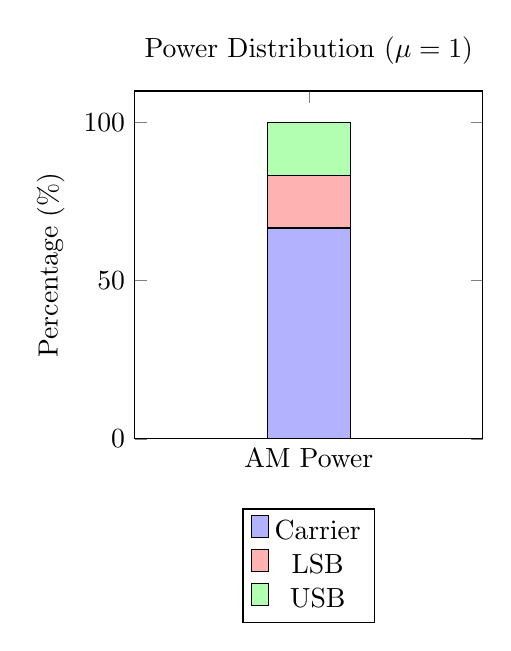
\begin{tikzpicture}
        \begin{axis}[
            ybar stacked,
            bar width=30pt,
            width=6cm, height=6cm,
            ymin=0, ymax=110,
            symbolic x coords={AM Power},
            xtick=data,
            ylabel={Percentage (\%)},
            title={Power Distribution ($\mu=1$)},
            legend style={at={(0.5,-0.2)}, anchor=north}
        ]
            \addplot[fill=blue!30] coordinates {(AM Power, 66.67)}; % Carrier
            \addplot[fill=red!30] coordinates {(AM Power, 16.66)}; % LSB
            \addplot[fill=green!30] coordinates {(AM Power, 16.66)}; % USB
            \legend{Carrier, LSB, USB}
        \end{axis}
    \end{tikzpicture}
    \captionof{figure}{Power Breakdown}
    \end{center}

    \begin{mnemonicbox}
    "CTTT" - Carrier Takes Two-Thirds
    \end{mnemonicbox}
\end{solutionbox}

\questionmarks{2}{b}{4}
\textbf{Why pre-emphases and de-emphases are used? Briefly describe how the signals are modified at transmitter side and receiver side.}

\begin{solutionbox}
    \textbf{Purpose of Pre-emphasis and De-emphasis:}
    
    Used primarily in FM to improve the Signal-to-Noise Ratio (SNR) for high-frequency components relative to the noise floor.

    \begin{itemize}
        \item \textbf{Improve SNR}: Boosts high frequencies before transmission to overcome noise.
        \item \textbf{Reduce Noise}: High frequencies in FM are more susceptible to noise.
        \item \textbf{Maintain Fidelity}: De-emphasis restores the original flat frequency response.
    \end{itemize}

    \textbf{Signal Modification Process:}

    \begin{center}
    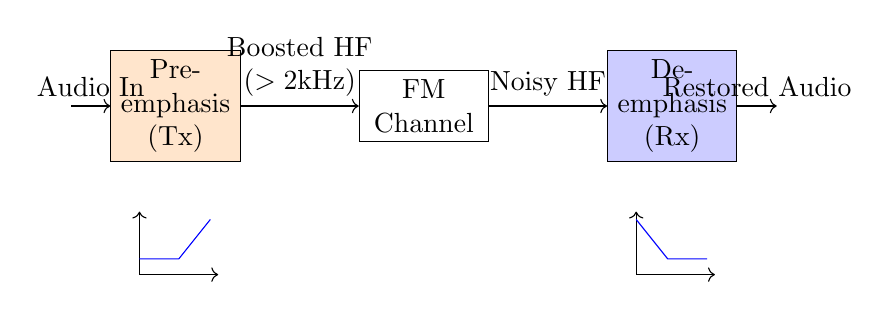
\begin{tikzpicture}[auto, node distance=1.5cm,
        block/.style={draw, rectangle, minimum height=2.5em, text width=4em, align=center},
        signal/.style={font=\footnotesize\itshape}
    ]
        \node [coordinate] (in) {};
        \node [block, right=0.5cm of in, fill=orange!20] (pre) {Pre-emphasis\\(Tx)};
        \node [block, right=1.5cm of pre] (ch) {FM\\Channel};
        \node [block, right=1.5cm of ch, fill=blue!20] (de) {De-emphasis\\(Rx)};
        \node [coordinate, right=0.5cm of de] (out) {};

        \draw [->] (in) -- node[above]{Audio In} (pre);
        \draw [->] (pre) -- node[above, align=center]{Boosted HF\\($>2$kHz)} (ch);
        \draw [->] (ch) -- node[above, align=center]{Noisy HF} (de);
        \draw [->] (de) -- node[above]{Restored Audio} (out);
        
        % Frequency response sketches
        \node [below=0.5cm of pre] {\tikz{\draw[->] (0,0) -- (1,0); \draw[->] (0,0) -- (0,0.8); \draw[blue] (0,0.2) -- (0.5,0.2) -- (0.9,0.7);}};
        \node [below=0.5cm of de] {\tikz{\draw[->] (0,0) -- (1,0); \draw[->] (0,0) -- (0,0.8); \draw[blue] (0,0.7) -- (0.4,0.2) -- (0.9,0.2);}};
    \end{tikzpicture}
    \captionof{figure}{Signal Modification Flow}
    \end{center}

    \begin{mnemonicbox}
    "BHCKO" - Boost High, Cut High, Keep Original
    \end{mnemonicbox}
\end{solutionbox}

\questionmarks{2}{c}{7}
\textbf{Explain FM generation techniques. Explain Phase locked loop FM modulator in detail.}

\begin{solutionbox}
    \textbf{FM Generation Techniques:}

    \begin{center}
    \begin{tabulary}{\linewidth}{L L L}
        \hline
        \textbf{Technique} & \textbf{Principle} & \textbf{Advantages} \\
        \hline
        Direct FM & Varying capacitance in oscillator (e.g., Varactor) & Simple design \\
        Indirect FM & Phase modulation to produce FM & Better frequency stability \\
        PLL FM & Using phase locked loop & High frequency stability \\
        Armstrong & Using mixers and multipliers & Excellent linearity \\
        \hline
    \end{tabulary}
    \captionof{table}{FM Generation Methods}
    \end{center}

    \textbf{PLL FM Modulator:}

    \begin{center}
    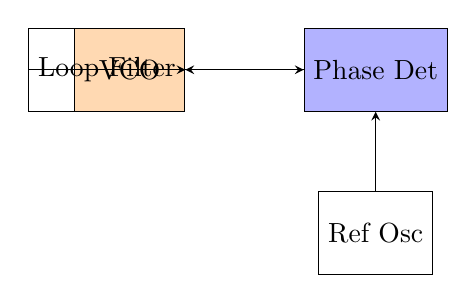
\begin{tikzpicture}[auto, node distance=2cm,
        block/.style={draw, rectangle, minimum height=3em, minimum width=4em, align=center},
        sum/.style={draw, circle, inner sep=0pt, minimum size=6mm},
        >=stealth
    ]
        % PLL Blocks
        \node [block, fill=orange!30] (vco) {VCO};
        \node [block, fill=blue!30, right=1.5cm of vco] (pd) {Phase Det};
        \node [block, below=1cm of pd] (ref) {Ref Osc};
        \node [block, left=1.5cm of pd] (lpf) {Loop Filter};

        % Connections
        \draw [->] (vco.east) -- (pd.west);
        \draw [->] (ref.north) -- (pd.south);
        \draw [->] (pd.west) -- (lpf.east);
        \draw [->] (lpf.west) -- (vco.east); % This is weird in block diagram layout, let's fix
        
        % Correcting layout for loop
        % Modulating signal enters VCO. Reference enters PD.
        % Actually, for FM Modulator using PLL:
        % The modulating signal is added to the loop error voltage before the VCO. 
        % OR modulating signal controls VCO directly in open loop? No, that's direct FM.
        
        % Standard PLL FM Modulator:
        % Use PLL to stabilize carrier. Modulating signal is added to the control voltage of VCO.
        % Or, Modulating signal is integrated and phase modulated?
        
        % Let's follow the MDX description: "Modulating signal directly controls the VCO".
        % Wait, if PLL is locked, it opposes change.
        % For PLL FM, the modulating signal is usually added to the error voltage driving the VCO.
        % The loop bandwidth must be low (lower than modulating freq) so loop doesn't cancel modulation.
    \end{tikzpicture}
    
    % Re-drawing based on typical PLL FM Modulator block
    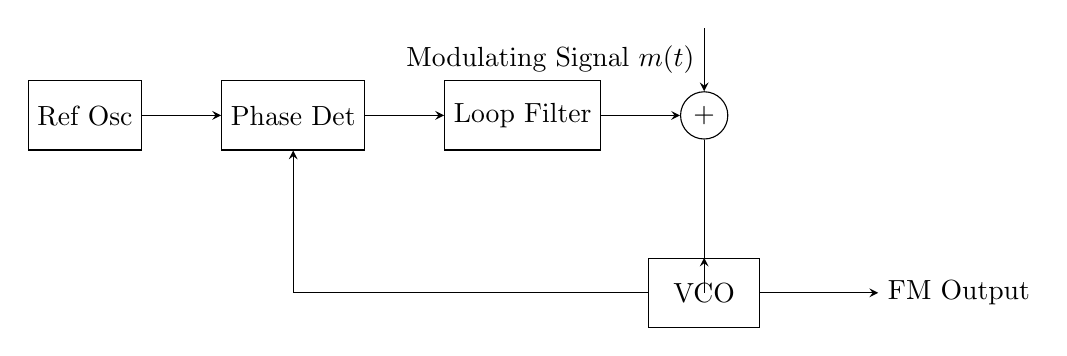
\begin{tikzpicture}[auto, node distance=1.5cm,
        block/.style={draw, rectangle, minimum height=2.5em, minimum width=4em, align=center},
        sum/.style={draw, circle, inner sep=0pt, minimum size=6mm},
        >=stealth
    ]
        \node [block] (ref) {Ref Osc};
        \node [block, right=1cm of ref] (pd) {Phase Det};
        \node [block, right=1cm of pd] (lpf) {Loop Filter};
        \node [sum, right=1cm of lpf] (adder) {+};
        \node [coordinate, above=0.8cm of adder] (mod_in) {};
        \node [block, below=1.5cm of adder] (vco) {VCO};
        \node [coordinate, right=1.5cm of vco] (out) {};

        \draw [->] (ref) -- (pd);
        \draw [->] (pd) -- (lpf);
        \draw [->] (lpf) -- (adder);
        \draw [->] (mod_in) -- node[left]{Modulating Signal $m(t)$} (adder);
        \draw [->] (adder) -- (vco.east -| adder.south) -- (vco.north); % connection to VCO input
        
        % VCO output goes to: 1. Output, 2. Phase Detector feedback
        \draw [->] (vco) -- (out) node[right]{FM Output};
        \draw [->] (vco.west) -| (pd.south);
        
    \end{tikzpicture}
    \captionof{figure}{PLL FM Modulator}
    \end{center}

    \textbf{Working Principle:}
    \begin{enumerate}
        \item \textbf{Phase Detector} compares VCO frequency with stable Reference Oscillator.
        \item \textbf{Loop Filter} provides DC control measure, blocking high frequency variations.
        \item \textbf{Modulating Signal} is added to the control voltage.
        \item This varies the \textbf{VCO} frequency according to message signal (FM).
        \item The PLL feedback ensures the center frequency remains stable (locked to reference) over long term, while allowing short-term deviations for modulation (if loop bandwidth is small).
    \end{enumerate}

    \begin{mnemonicbox}
    "PDCFV" - Phase Detector Compares, Filter Smooths, VCO Varies
    \end{mnemonicbox}
\end{solutionbox}

\questionmarks{2}{a}{3}
\textbf{State advantages and disadvantage of SSB over DSB.}

\begin{solutionbox}
    \textbf{Advantages and Disadvantages of SSB over DSB:}

    \begin{center}
    \begin{tabulary}{\linewidth}{L L}
        \hline
        \textbf{Advantages of SSB} & \textbf{Disadvantages of SSB} \\
        \hline
        \textbf{Bandwidth Efficiency}: Uses only half bandwidth ($f_m$) compared to DSB. & \textbf{Complex Circuitry}: Requires sharp filters for sideband suppression. \\
        \textbf{Power Efficiency}: Uses about 1/3 to 1/6 power for same SNR. & \textbf{Difficult Demodulation}: Requires precise carrier re-insertion (coherent detection). \\
        \textbf{Reduced Fading}: Less susceptible to selective fading. & \textbf{Low Freq Distortion}: Practical filters attenuate low frequencies. \\
        \textbf{Less Interference}: Narrower channel usage. & \textbf{Cost}: Higher transmitter/receiver cost. \\
        \hline
    \end{tabulary}
    \captionof{table}{SSB vs DSB}
    \end{center}

    \begin{mnemonicbox}
    "PBSCN" - Power and Bandwidth Saved, But Complex Circuits Needed
    \end{mnemonicbox}
\end{solutionbox}

\questionmarks{2}{b}{4}
\textbf{Sketch the frequency spectrum of DSBSC and SSB amplitude modulated wave and pilot carrier.}

\begin{solutionbox}
    \textbf{Frequency Spectrum Comparison:}

    \begin{center}
    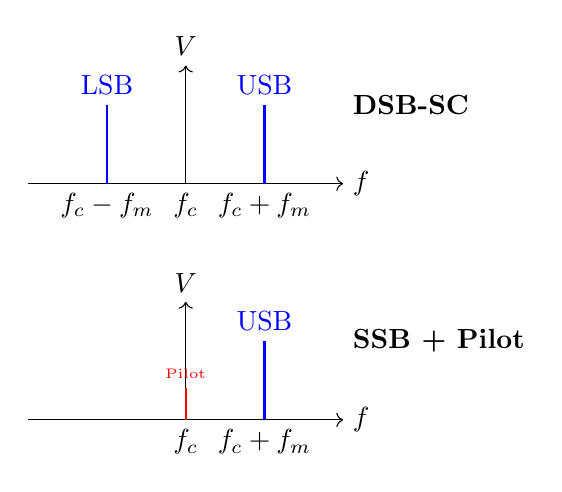
\begin{tikzpicture}
        % DSBSC
        \begin{scope}[yshift=3cm]
            \draw[->] (-2,0) -- (2,0) node[right] {$f$};
            \draw[->] (0,0) -- (0,1.5) node[above] {$V$};
            \node[right] at (2,1) {\textbf{DSB-SC}};
            \draw[thick, blue] (-1,0) -- (-1,1) node[above]{LSB};
            \draw[thick, blue] (1,0) -- (1,1) node[above]{USB};
            \node[below] at (0,0) {$f_c$};
            \node[below] at (-1,0) {$f_c-f_m$};
            \node[below] at (1,0) {$f_c+f_m$};
        \end{scope}

        % SSB with Pilot
        \begin{scope}[yshift=0cm]
            \draw[->] (-2,0) -- (2,0) node[right] {$f$};
            \draw[->] (0,0) -- (0,1.5) node[above] {$V$};
            \node[right] at (2,1) {\textbf{SSB + Pilot}};
            
            \draw[thick, blue] (1,0) -- (1,1) node[above]{USB};
            \draw[thick, red] (0,0) -- (0,0.4) node[above, font=\tiny]{Pilot};
            
            \node[below] at (0,0) {$f_c$};
            \node[below] at (1,0) {$f_c+f_m$};
        \end{scope}
    \end{tikzpicture}
    \captionof{figure}{DSB-SC vs SSB with Pilot Carrier Spectrum}
    \end{center}

    \begin{itemize}
        \item \textbf{DSB-SC}: Carrier suppressed, inputs power only in sidebands. Bandwidth $2f_m$.
        \item \textbf{SSB + Pilot}: Only one sideband transmitted + reduced carrier for synchronization. Bandwidth $f_m$.
    \end{itemize}

    \begin{mnemonicbox}
    "TSOSP" - Two Sides, One Side, or One Side Plus Pilot
    \end{mnemonicbox}
\end{solutionbox}

\questionmarks{2}{c}{7}
\textbf{Write a short-note on: Pulse modulation.}

\begin{solutionbox}
    \textbf{Pulse Modulation Techniques:}
    
    Process where continuous analog signal is sampled and converted into pulses parameters.

    \begin{center}
    \begin{tabulary}{\linewidth}{L L L}
        \hline
        \textbf{Type} & \textbf{Principle} & \textbf{Application} \\
        \hline
        \textbf{PAM} & Amplitude of pulses varies with signal & TDM, intermediate step for PCM \\
        \textbf{PWM} & Width/duration of pulses varies & Motor control, power delivery \\
        \textbf{PPM} & Position/timing of pulses varies & Optical communication, RF control \\
        \textbf{PCM} & Digital binary code representation & Computing, Digital Audio, Telephony \\
        \hline
    \end{tabulary}
    \captionof{table}{Pulse Modulation Types}
    \end{center}

    \textbf{Waveform Comparison:}

    \begin{center}
    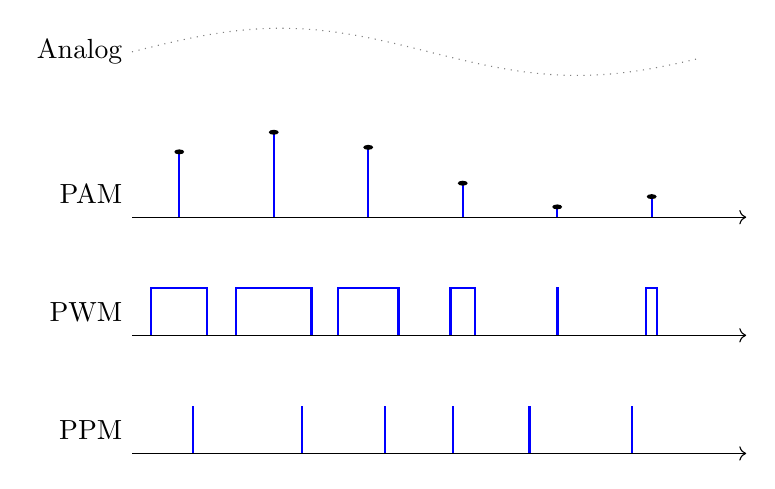
\begin{tikzpicture}[xscale=1.2, yscale=0.6]
        % Analog
        \draw[gray, dotted] plot[domain=0:6, samples=50] (\x, {1 + 0.5*sin(deg(\x))});
        \node[left] at (0,1) {Analog};
        
        % PAM
        \begin{scope}[yshift=-2.5cm]
            \foreach \x in {0.5, 1.5, ..., 5.5} {
                \draw[thick, blue] (\x, 0) -- (\x, {1 + 0.8*sin(deg(\x))});
                \fill (\x, {1 + 0.8*sin(deg(\x))}) circle (1.5pt);
            }
            \draw[->] (0,0) -- (6.5,0);
            \node[left] at (0,0.5) {PAM};
        \end{scope}

        % PWM
        \begin{scope}[yshift=-5cm]
            \foreach \x in {0.5, 1.5, ..., 5.5} {
                \pgfmathsetmacro{\w}{0.2 + 0.2*sin(deg(\x))}
                \draw[thick, blue] (\x-\w, 0) -- (\x-\w, 1) -- (\x+\w, 1) -- (\x+\w, 0);
            }
            \draw[->] (0,0) -- (6.5,0);
            \node[left] at (0,0.5) {PWM};
        \end{scope}

        % PPM
        \begin{scope}[yshift=-7.5cm]
             \foreach \x in {0.5, 1.5, ..., 5.5} {
                \pgfmathsetmacro{\s}{0.3*sin(deg(\x))}
                \draw[thick, blue] (\x+\s, 0) -- (\x+\s, 1);
            }
            \draw[->] (0,0) -- (6.5,0);
            \node[left] at (0,0.5) {PPM};
        \end{scope}
    \end{tikzpicture}
    \captionof{figure}{Pulse Modulation Waveforms}
    \end{center}

    \begin{mnemonicbox}
    "AWPC" - Amplitude, Width, Position, Code - All Pulse Types
    \end{mnemonicbox}
\end{solutionbox}

\questionmarks{3}{a}{3}
\textbf{What is AGC? Draw and explain input-output characteristic curve of simple AGC circuit.}

\begin{solutionbox}
    \textbf{Automatic Gain Control (AGC):}
    \begin{itemize}
        \item \textbf{Definition}: A circuit that automatically adjusts receiver gain to maintain a relatively constant output signal level despite variations in input signal strength.
        \item \textbf{Purpose}: Prevents overloading on strong signals and fading on weak signals.
    \end{itemize}

    \textbf{Input-Output Characteristics:}

    \begin{center}
    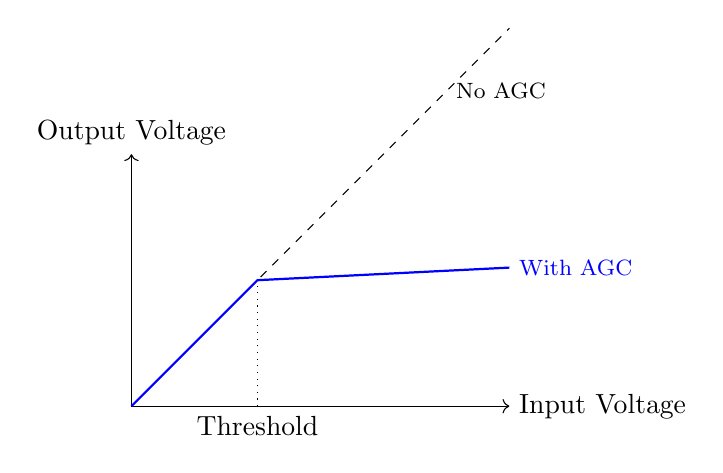
\begin{tikzpicture}[scale=0.8]
        \draw[->] (0,0) -- (6,0) node[right] {Input Voltage};
        \draw[->] (0,0) -- (0,4) node[above] {Output Voltage};
        
        \draw[dashed] (0,0) -- (2,2) -- (6,6); % Linear / No AGC
        \node[right, font=\footnotesize] at (5,5) {No AGC};
        
        \draw[thick, blue] (0,0) -- (2,2) -- (6,2.2); % With AGC
        \node[right, blue, font=\footnotesize] at (6,2.2) {With AGC};
        
        \draw[dotted] (2,0) -- (2,2);
        \node[below] at (2,0) {Threshold};
    \end{tikzpicture}
    \captionof{figure}{AGC Characteristics}
    \end{center}

    \textbf{Explanation}: Linear response for weak signals (below threshold). Above threshold, gain is reduced to flatten output.

    \begin{mnemonicbox}
    "SSLG" - Strong Signals Get Less Gain
    \end{mnemonicbox}
\end{solutionbox}

\questionmarks{3}{b}{4}
\textbf{Write a short-note on balanced ratio detector for FM demodulation.}

\begin{solutionbox}
    \textbf{Balanced Ratio Detector:}

    \begin{itemize}
        \item FM demodulator deriving output from the ratio of diode currents.
        \item \textbf{Key Components}: Center-tapped transformer, two diodes, large electrolytic capacitor (for AM rejection).
        \item \textbf{Advantage}: Provides inherent immunity to Amplitude variations (AM Rejection) without a separate limiter.
    \end{itemize}

    \textbf{Circuit Diagram:}

    \begin{center}
    \begin{circuitikz}[font=\footnotesize]
        \draw (0,0) node[left]{FM In} to[L] (0,-2);
        \draw (1.5,0) to[L] (1.5,-2);
        \draw (1.5,-1) -- (2.5,-1); % Primary link or center tap
        
        % Diodes in Ratio Detector point in same loop direction usually
        % But standard layout: Top diode > right, Bottom diode < left? No that's discriminator.
        % Ratio Detector:
        % Secondary Top -> Diode -> Load -> | <- Load <- Diode <- Secondary Bottom
        
        \draw (1.5,0) -- (2.5,0) to[diode, l=$D_1$] (4.5,0);
        \draw (1.5,-2) -- (2.5,-2) to[diode, l=$D_2$, invert] (4.5,-2);
        
        % Load capacitors and resistors
        \draw (4.5,0) to[C, l=$C_1$] (4.5,-1) coordinate (mid);
        \draw (4.5,-2) to[C, l=$C_2$] (mid);
        
        % Resistors for load
        % Large capacitor C_L across both
        \draw (4.5,0) -- (6,0) to[C, l=$C_L$ (Large)] (6,-2) -- (4.5,-2);
        
        % Output taken from center
        \draw (mid) -- (6,-1) node[right] {Output};
        
        % Tertiary winding coupling
        \draw (2.5,-1) to[L] (1,-1) to[C] (0,-1); % Loose coupling representation
    \end{circuitikz}
    \captionof{figure}{Ratio Detector Circuit}
    \end{center}

    \begin{mnemonicbox}
    "BDTFV" - Balanced Diodes Transform Frequency To Voltage
    \end{mnemonicbox}
\end{solutionbox}

\questionmarks{3}{c}{7}
\textbf{Explain working of various types of FM demodulator circuits.}

\begin{solutionbox}
    \textbf{Types of FM Demodulators:}

    \begin{center}
    \begin{tabulary}{\linewidth}{L L L}
        \hline
        \textbf{Type} & \textbf{Working Principle} & \textbf{Pros/Cons} \\
        \hline
        \textbf{Slope Detector} & Uses non-linear region of tuned circuit & Simple / Poor linearity \\
        \textbf{Foster-Seeley} & Phase shift differentiation & Good linearity / No AM rejection \\
        \textbf{Ratio Detector} & Ratio of diode voltages & Good AM rejection / Med linearity \\
        \textbf{PLL Demodulator} & Phase locking to input & Excellent linearity / Complex \\
        \textbf{Quadrature} & Phase shift \& multiplication & Easy IC integration \\
        \hline
    \end{tabulary}
    \captionof{table}{FM Demodulator Types}
    \end{center}

    \textbf{PLL FM Demodulator Diagram:}

    \begin{center}
    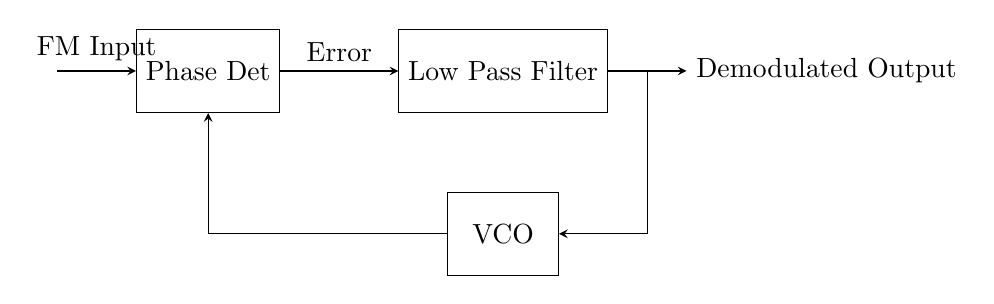
\begin{tikzpicture}[auto, node distance=1.5cm,
        block/.style={draw, rectangle, minimum height=3em, minimum width=4em, align=center},
        >=stealth
    ]
        \node [block] (pd) {Phase Det};
        \node [block, right=1.5cm of pd] (lpf) {Low Pass Filter};
        \node [block, below=1cm of lpf] (vco) {VCO};
        \node [coordinate, left=1cm of pd] (in) {};
        \node [coordinate, right=1cm of lpf] (out) {};

        \draw [->] (in) -- node[above]{FM Input} (pd);
        \draw [->] (pd) -- node[above]{Error} (lpf);
        \draw [->] (lpf) -- coordinate (tap) (out) node[right]{Demodulated Output};
        \draw [->] (tap) |- (vco);
        \draw [->] (vco) -| (pd);
    \end{tikzpicture}
    \captionof{figure}{PLL Demodulator}
    \end{center}

    \textbf{Working:} The error voltage required to keep the VCO locked to the input FM signal is proportional to the frequency deviation, thus recovering the original message.

    \begin{mnemonicbox}
    "FVDPE" - Frequency Variations Drive Phase Errors
    \end{mnemonicbox}
\end{solutionbox}


\questionmarks{3}{a}{3} % OR
\textbf{Explain characteristics of a Radio receiver.}

\begin{solutionbox}
    \textbf{Characteristics of a Radio Receiver:}

    \begin{center}
    \begin{tabulary}{\linewidth}{L L L}
        \hline
        \textbf{Characteristic} & \textbf{Definition} & \textbf{Importance} \\
        \hline
        \textbf{Sensitivity} & Ability to amplify weak signals & Determines maximum reception range \\
        \textbf{Selectivity} & Ability to separate desired signal from adjacent signals & Prevents interference \\
        \textbf{Fidelity} & Accuracy in reproducing original signal & Ensures sound quality \\
        \textbf{Image Rejection} & Ability to reject image frequency & Prevents duplicate reception \\
        \hline
    \end{tabulary}
    \captionof{table}{Receiver Specifications}
    \end{center}

    \begin{center}
    \begin{tikzpicture}[
        mindmap, concept color=blue!20,
        every node/.style={concept, scale=0.8},
        grow cyclic,
        level 1/.style={level distance=3cm, sibling angle=90}
    ]
        \node [concept color=orange!40] {Receiver\\Characteristics}
        child { node {Sensitivity} }
        child { node {Selectivity} }
        child { node {Fidelity} }
        child { node {Image Rejection} };
    \end{tikzpicture}
    \captionof{figure}{Key Characteristics}
    \end{center}

    \begin{mnemonicbox}
    "SSFIM" - Select Signals Faithfully, Ignore Mirrors
    \end{mnemonicbox}
\end{solutionbox}

\questionmarks{3}{b}{4} % OR
\textbf{Explain types of distortions occur in AM detector circuit.}

\begin{solutionbox}
    \textbf{Distortions in AM Detector:}

    \begin{center}
    \begin{tabulary}{\linewidth}{L L L}
        \hline
        \textbf{Distortion} & \textbf{Cause} & \textbf{Remedy} \\
        \hline
        Diagonal Clipping & RC time constant too large (cant discharge fast enough) & Reduce R or C \\
        Negative Peak Clipping & Modulation index high + AC/DC load mismatch & Adjust biasing / load \\
        Harmonic Distortion & Non-linear diode characteristics & Better diodes \\
        \hline
    \end{tabulary}
    \captionof{table}{AM Detector Distortions}
    \end{center}

    \textbf{Waveforms:}

    \begin{center}
    \begin{tikzpicture}[xscale=2, yscale=1]
        % Normal
        \draw[gray, dotted] plot[domain=0:2*pi] (\x, {1 + 0.5*sin(deg(\x))});
        
        % Diagonal Clipping
        \begin{scope}[yshift=-2.5cm]
            \draw[->] (0,0) -- (6.5,0);
            \node[left] at (0,0.5) {Diagonal};
            \draw[thick, red] (0,1) -- (0.5,1.4) -- (1.5,0.8) -- (2.0,1.4); % Rough sketch of clipping
            % Better approximation of diagonal clipping (exponential decay slower than sine)
            \draw[blue] plot[domain=0:6] (\x, {1 + 0.5*sin(deg(\x))});
            \draw[red, thick] (1.6, 1.5) -- (2.5, 0.8); % The "diagonal" part
        \end{scope}

        % Negative Peak Clipping
        \begin{scope}[yshift=-5cm]
            \draw[->] (0,0) -- (6.5,0);
            \node[left] at (0,0.5) {Negative Peak};
            \draw[blue] plot[domain=0:6] (\x, {1 + 0.8*sin(deg(\x))});
            \draw[red, thick] (3.5, 0) -- (5.5, 0); % Flat bottom
        \end{scope}
    \end{tikzpicture}
    \captionof{figure}{Distortion Types}
    \end{center}

    \begin{mnemonicbox}
    "DNHF" - Diagonal Negative Harmonics Frequency
    \end{mnemonicbox}
\end{solutionbox}

\questionmarks{3}{c}{7} % OR
\textbf{Draw the block diagram of a Superheterodyne AM receiver and explain it.}

\begin{solutionbox}
    \textbf{Superheterodyne AM Receiver:}

    \begin{center}
    \begin{tikzpicture}[auto, node distance=1.5cm,
        block/.style={draw, rectangle, minimum height=3em, minimum width=3.5em, align=center},
        >=stealth
    ]
        \node [coordinate] (ant) {};
        \node [block, right=0.5cm of ant] (rf) {RF Amp};
        \node [block, right=1cm of rf] (mix) {Mixer};
        \node [block, below=1cm of mix] (lo) {Local Osc};
        \node [block, right=1cm of mix] (if) {IF Amp};
        \node [block, right=1cm of if] (det) {Detector};
        \node [block, right=1cm of det] (af) {AF Amp};
        \node [coordinate, right=0.5cm of af] (spk) {};
        \node [block, above=1cm of if] (agc) {AGC};

        \draw [->] (ant) -- node[above]{Antenna} (rf);
        % If antenna image missing, use text or TikZ antenna
        % \draw [->] (ant) -- (rf); 
        \draw [->] (rf) -- (mix);
        \draw [->] (lo) -- (mix);
        \draw [->] (mix) -- node[above]{IF} (if);
        \draw [->] (if) -- (det);
        \draw [->] (det) -- (af);
        \draw [->] (af) -- node[right]{Speaker} (spk);
        
        \draw [->] (det.north) |- (agc.east);
        \draw [->] (agc.west) -| (rf.north);
        \draw [->] (agc.south) -- (if.north);

    \end{tikzpicture}
    \captionof{figure}{Superheterodyne Receiver}
    \end{center}

    \textbf{Function of Blocks:}
    \begin{tabulary}{\linewidth}{L L}
        \textbf{RF Amp}: Selects and amplifies desired RF signal. \\
        \textbf{Mixer}: Mixes RF ($f_s$) and LO ($f_o$) to produce IF ($f_o - f_s$). \\
        \textbf{IF Amp}: Main amplification stage at fixed Intermediate Frequency (455 kHz). \\
        \textbf{Detector}: Demodulates AM signal to Audio. \\
        \textbf{AGC}: Maintains constant volume.
    \end{tabulary}

    \begin{mnemonicbox}
    "RMLIDAS" - Radio Mixing Local Intermediate Detected Audio Signals
    \end{mnemonicbox}
\end{solutionbox}

\questionmarks{4}{a}{3}
\textbf{Explain quantization process used in analog to digital conversion.}

\begin{solutionbox}
    \textbf{Quantization Process:}
    \begin{enumerate}
        \item \textbf{Sampling}: Discretize time.
        \item \textbf{Level Allocation}: Divide amplitude range into $L$ discrete levels.
        \item \textbf{Assignment}: Map each sample value to nearest level.
        \item \textbf{Encoding}: Convert level index to binary.
    \end{enumerate}

    \begin{center}
    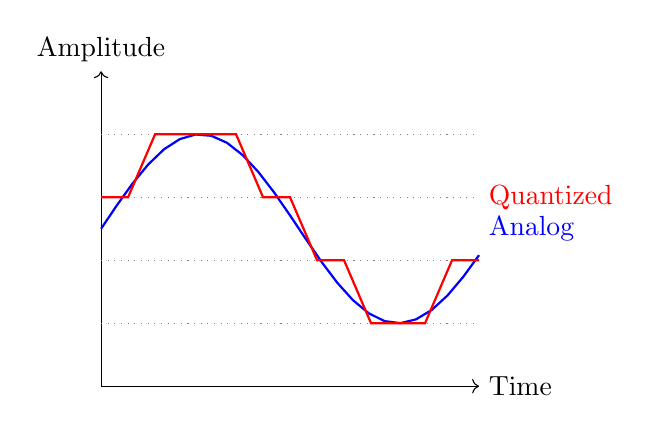
\begin{tikzpicture}[scale=0.8]
        \draw[->] (0,0) -- (6,0) node[right]{Time};
        \draw[->] (0,0) -- (0,5) node[above]{Amplitude};
        
        \foreach \y in {1,2,3,4} \draw[gray, dotted] (0,\y) -- (6,\y);
        
        \draw[blue, thick] plot[domain=0:6] (\x, {2.5 + 1.5*sin(deg(\x))});
        \draw[red, thick, step=0.5] plot[domain=0:6, samples=15] (\x, {round(2.5 + 1.5*sin(deg(\x)))});
        
        \node[right, blue] at (6, 2.5) {Analog};
        \node[right, red] at (6, 3) {Quantized};
    \end{tikzpicture}
    \captionof{figure}{Quantization Staircase}
    \end{center}

    \begin{mnemonicbox}
    "SLAB" - Sample Levels Assign Binary
    \end{mnemonicbox}
\end{solutionbox}

\questionmarks{4}{b}{4}
\textbf{Give the comparison of Sampling techniques.}

\begin{solutionbox}
    \textbf{Sampling Techniques:}

    \begin{center}
    \begin{tabulary}{\linewidth}{L L L}
        \hline
        \textbf{Technique} & \textbf{Description} & \textbf{Pros/Cons} \\
        \hline
        Ideal & Instantaneous impulses & Theoretical only \\
        Natural & Pulse top follows signal shape & Complex generation \\
        Flat-top & Pulse top is flat (Sample \& Hold) & Easy to generate / Aperture error \\
        \hline
    \end{tabulary}
    \captionof{table}{Sampling Types}
    \end{center}

    \begin{center}
    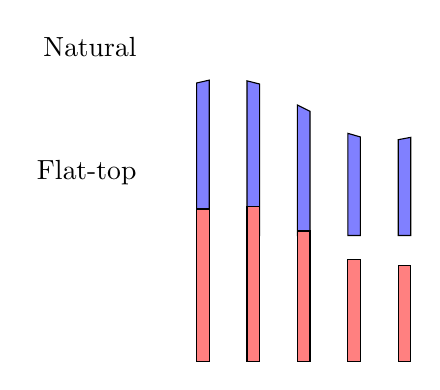
\begin{tikzpicture}[scale=0.8]
        \node[left] at (0,3) {Natural};
        \foreach \x in {1,2,3,4,5} {
             \draw[fill=blue!50] (0.8*\x, 0) -- (0.8*\x, {2+0.5*sin(deg(\x))}) -- (0.8*\x+0.2, {2+0.5*sin(deg(\x+0.2))}) -- (0.8*\x+0.2, 0) -- cycle;
        }

        \node[left] at (0,1) {Flat-top};
        \foreach \x in {1,2,3,4,5} {
             \draw[fill=red!50] (0.8*\x, -2) rectangle (0.8*\x+0.2, {0.5*sin(deg(\x))});
        }
    \end{tikzpicture}
    \captionof{figure}{Natural vs Flat-top Sampling}
    \end{center}

    \begin{mnemonicbox}
    "INF" - Ideal Natural Flat
    \end{mnemonicbox}
\end{solutionbox}

\questionmarks{4}{c}{7}
\textbf{Draw and explain block diagram of a PCM transmitter and receiver.}

\begin{solutionbox}
    \textbf{Pulse Code Modulation (PCM):}

    \textbf{Transmitter:}
    \begin{center}
    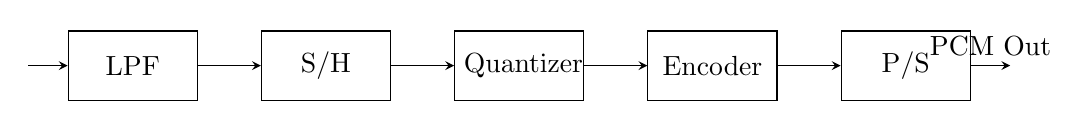
\begin{tikzpicture}[auto, node distance=1.2cm,
        block/.style={draw, rectangle, minimum height=2.5em, text width=4em, align=center},
        >=stealth
    ]
        \node[coordinate](in){};
        \node[block, right=0.5cm of in](lpf){LPF};
        \node[block, right=0.8cm of lpf](sh){S/H};
        \node[block, right=0.8cm of sh](q){Quantizer};
        \node[block, right=0.8cm of q](enc){Encoder};
        \node[block, right=0.8cm of enc](p2s){P/S};
        \node[coordinate, right=0.5cm of p2s](out){};

        \draw[->] (in) -- (lpf);
        \draw[->] (lpf) -- (sh);
        \draw[->] (sh) -- (q);
        \draw[->] (q) -- (enc);
        \draw[->] (enc) -- (p2s);
        \draw[->] (p2s) -- node[above]{PCM Out} (out);
    \end{tikzpicture}
    \end{center}

    \textbf{Receiver:}
    \begin{center}
    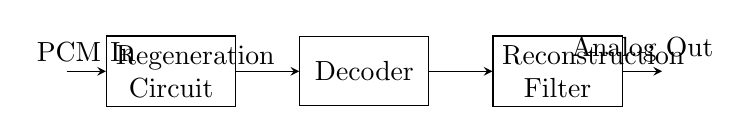
\begin{tikzpicture}[auto, node distance=1.2cm,
        block/.style={draw, rectangle, minimum height=2.5em, text width=4em, align=center},
        >=stealth
    ]
        \node[coordinate](in){};
        \node[block, right=0.5cm of in](regen){Regeneration\\Circuit};
        \node[block, right=0.8cm of regen](dec){Decoder};
        \node[block, right=0.8cm of dec](recon){Reconstruction\\Filter};
        \node[coordinate, right=0.5cm of recon](out){};

        \draw[->] (in) -- node[above]{PCM In} (regen);
        \draw[->] (regen) -- (dec);
        \draw[->] (dec) -- (recon);
        \draw[->] (recon) -- node[above]{Analog Out} (out);
    \end{tikzpicture}
    \end{center}

    \begin{mnemonicbox}
    "FSQEMT" - Filter, Sample, Quantize, Encode, Multiplex, Transmit
    \end{mnemonicbox}
\end{solutionbox}

\questionmarks{4}{a}{3} % OR
\textbf{State and explain Nyquist theorem.}

\begin{solutionbox}
    \textbf{Nyquist Sampling Theorem:}
    To perfectly reconstruct a band-limited signal, the sampling frequency $f_s$ must be at least twice the maximum frequency component $f_{max}$ present in the signal.
    \[ f_s \ge 2 f_{max} \]
    
    \begin{itemize}
        \item $2f_{max}$ is called the \textbf{Nyquist Rate}.
        \item If $f_s < 2f_{max}$, \textbf{Aliasing} occurs (overlapping of spectral components).
    \end{itemize}

    \begin{center}
    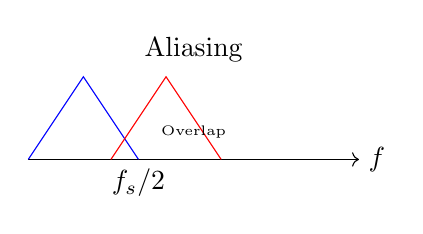
\begin{tikzpicture}[scale=0.7]
        % Aliasing
        \draw[->] (0,0) -- (6,0) node[right]{$f$};
        \node at (3,2) {Aliasing};
        \draw[blue] (0,0) -- (1,1.5) -- (2,0);
        \draw[red] (1.5,0) -- (2.5,1.5) -- (3.5,0);
        \node[below] at (2,0) {$f_s/2$};
        \node[font=\tiny] at (3,0.5) {Overlap};
    \end{tikzpicture}
    \captionof{figure}{Effect of Undersampling (Aliasing)}
    \end{center}

    \begin{mnemonicbox}
    "DMFSA" - Double Maximum Frequency Stops Aliasing
    \end{mnemonicbox}
\end{solutionbox}

\questionmarks{4}{b}{4} % OR
\textbf{Compare DM, ADM and DPCM.}

\begin{solutionbox}
    \textbf{Comparison:}

    \begin{center}
    \begin{tabulary}{\linewidth}{L L L L}
        \hline
        \textbf{Feature} & \textbf{Delta Mod (DM)} & \textbf{Adaptive DM} & \textbf{DPCM} \\
        \hline
        \textbf{Bits/Sample} & 1 Bit & 1 Bit & $>$ 1 Bit \\
        \textbf{Step Size} & Fixed & Variable & Fixed/Adaptive \\
        \textbf{Errors} & Slope Overload, Granular & Reduced errors & Quantization noise \\
        \textbf{Complexity} & Lowest & Moderate & High \\
        \hline
    \end{tabulary}
    \captionof{table}{DM vs ADM vs DPCM}
    \end{center}

    \begin{mnemonicbox}
    "SAMD" - Single-bit, Adaptive-bit, Multi-bit Difference
    \end{mnemonicbox}
\end{solutionbox}

\questionmarks{4}{c}{7} % OR
\textbf{Explain working of Differential PCM (DPCM) transmitter and receiver.}

\begin{solutionbox}
    \textbf{DPCM Principle:}
    Encodes the \textit{difference} between the actual sample and a predicted value (based on previous samples) rather than the absolute sample value.

    \textbf{DPCM Transmitter:}
    \begin{center}
    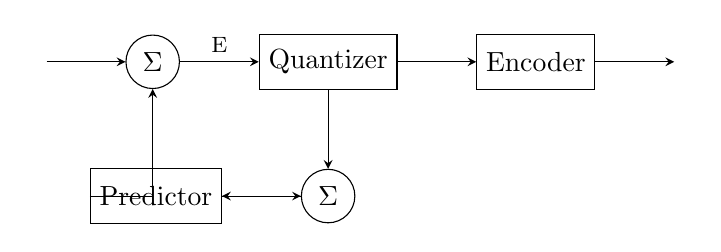
\begin{tikzpicture}[auto, node distance=1.5cm, >=stealth]
        \node[draw, rectangle, minimum height=2em] (quant) {Quantizer};
        \node[draw, rectangle, minimum height=2em, right=1cm of quant] (enc) {Encoder};
        \node[right=1cm of enc] (out) {};
        
        \node[draw, circle, left=1cm of quant] (sub) {$\Sigma$};
        \node[left=1cm of sub] (in) {};
        
        \node[draw, circle, below=1cm of quant] (add) {$\Sigma$};
        \node[draw, rectangle, minimum height=2em, left=1cm of add] (pred) {Predictor};
        
        \draw[->] (in) -- (sub);
        \draw[->] (sub) -- node[above]{\footnotesize E} (quant);
        \draw[->] (quant) -- (enc);
        \draw[->] (enc) -- (out);
        
        \draw[->] (quant) -- (add);
        \draw[->] (add) -- (pred);
        \draw[->] (pred) -| (sub);
        \draw[->] (pred) -- (add);
    \end{tikzpicture}
    \captionof{figure}{DPCM Transmitter}
    \end{center}

    \textbf{DPCM Receiver:}
    \begin{center}
    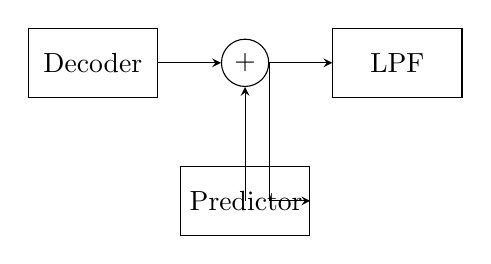
\begin{tikzpicture}[auto, node distance=1.5cm,
        block/.style={draw, rectangle, minimum height=2.5em, text width=4em, align=center},
        sum/.style={draw, circle, inner sep=0pt, minimum size=6mm},
        >=stealth
    ]
        \node[block](dec){Decoder};
        \node[sum, right=0.8cm of dec](sum){+};
        \node[block, below=1cm of sum](pred){Predictor};
        \node[block, right=0.8cm of sum](lpf){LPF};
        
        \draw[->] (dec) -- (sum);
        \draw[->] (sum) -- (lpf);
        \draw[->] (sum.east) |- (pred.east); % Feed output back
        \draw[->] (pred) -| (sum.south);
    \end{tikzpicture}
    \captionof{figure}{DPCM Receiver}
    \end{center}

    \begin{mnemonicbox}
    "PSQD" - Predict Subtract Quantize Difference
    \end{mnemonicbox}
\end{solutionbox}

\questionmarks{5}{a}{3}
\textbf{Describe TDMA frame.}

\begin{solutionbox}
    \textbf{TDMA Frame Structure:}

    Time Division Multiple Access allows multiple users to share same frequency by allocating unique time slots.

    \begin{center}
    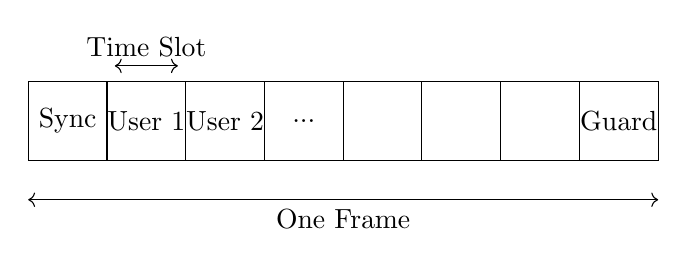
\begin{tikzpicture}
        \draw (0,0) rectangle (8,1);
        \foreach \x in {1,2,3,4,5,6,7} \draw (\x,0) -- (\x,1);
        \node at (0.5,0.5) {Sync};
        \node at (1.5,0.5) {User 1};
        \node at (2.5,0.5) {User 2};
        \node at (3.5,0.5) {...};
        \node at (7.5,0.5) {Guard};
        
        \draw[<->] (0, -0.5) -- (8,-0.5) node[midway, below] {One Frame};
        \draw[<->] (1.1, 1.2) -- (1.9, 1.2) node[midway, above] {Time Slot};
    \end{tikzpicture}
    \captionof{figure}{TDMA Frame}
    \end{center}

    Components: Preamble (Sync), Information Message, Guard Bits (Gap).

    \begin{mnemonicbox}
    "SITDA" - Slots In Time Divide Access
    \end{mnemonicbox}
\end{solutionbox}

\questionmarks{5}{b}{4}
\textbf{Draw and explain 4 level digital multiplexing hierarchies.}

\begin{solutionbox}
    \textbf{Digital Multiplexing Hierarchy (North American T-carrier):}

    \begin{center}
    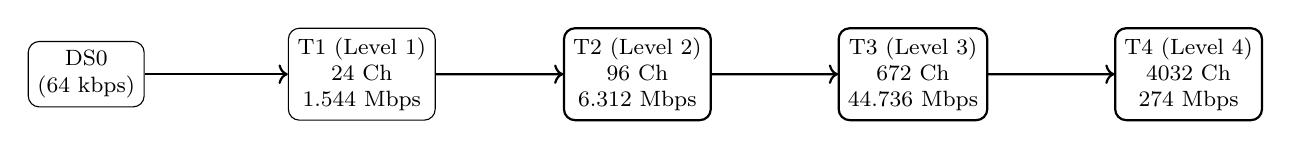
\begin{tikzpicture}[
        grow=right,
        level 1/.style={level distance=3.5cm, sibling distance=2cm},
        level 2/.style={level distance=3.5cm, sibling distance=1.5cm},
        edge from parent/.style={draw, ->, thick},
        every node/.style={draw, rectangle, rounded corners, align=center, font=\footnotesize}
    ]
        \node {DS0\\(64 kbps)}
            child {
                node {T1 (Level 1)\\24 Ch\\1.544 Mbps}
                child {
                    node {T2 (Level 2)\\96 Ch\\6.312 Mbps}
                    child {
                        node {T3 (Level 3)\\672 Ch\\44.736 Mbps}
                        child {
                            node {T4 (Level 4)\\4032 Ch\\274 Mbps}
                        }
                    }
                }
            };
    \end{tikzpicture}
    \captionof{figure}{T-Carrier Hierarchy}
    \end{center}

    \begin{mnemonicbox}
    "PSTQ" - Primary, Secondary, Tertiary, Quaternary Levels
    \end{mnemonicbox}
\end{solutionbox}

\questionmarks{5}{c}{7}
\textbf{Draw and explain block diagram of PCM-TDM system.}

\begin{solutionbox}
    \textbf{PCM-TDM Block Diagram:}

    \begin{center}
    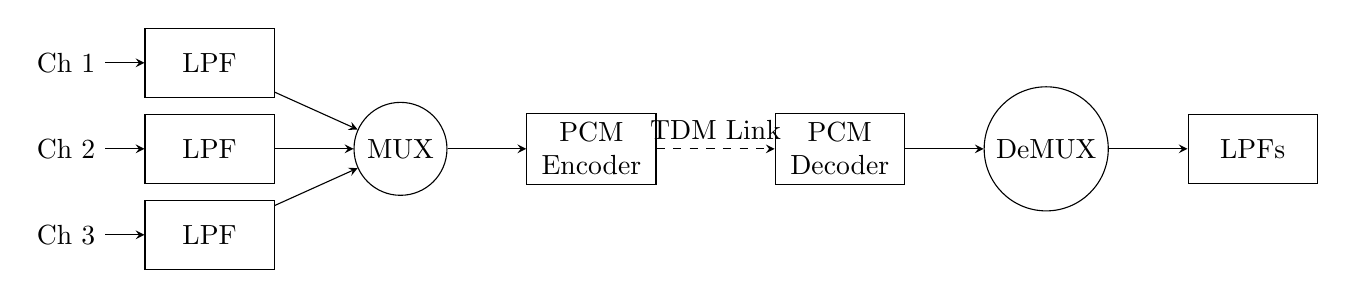
\begin{tikzpicture}[auto, node distance=1.2cm,
        block/.style={draw, rectangle, minimum height=2.5em, text width=4em, align=center},
        >=stealth
    ]
        % Inputs
        \node (in1) {Ch 1};
        \node [below=0.6cm of in1] (in2) {Ch 2};
        \node [below=0.6cm of in2] (in3) {Ch 3};
        
        % LPFs
        \node [block, right=0.5cm of in1] (lpf1) {LPF};
        \node [block, right=0.5cm of in2] (lpf2) {LPF};
        \node [block, right=0.5cm of in3] (lpf3) {LPF};
        
        % Commutator (Sampler/MUX)
        \node [draw, circle, right=1cm of lpf2, minimum size=1cm] (mux) {MUX};
        
        % PCM Blocks
        \node [block, right=1cm of mux] (pcm) {PCM Encoder};
        \node [coordinate, right=0.5cm of pcm] (tx) {};
        
        % Rx side
        \node [block, right=1.5cm of pcm] (dec) {PCM Decoder};
        \node [draw, circle, right=1cm of dec, minimum size=1cm] (demux) {DeMUX};
        \node [block, right=1cm of demux] (lpf_out) {LPFs};
        
        \draw[->] (in1) -- (lpf1);
        \draw[->] (in2) -- (lpf2);
        \draw[->] (in3) -- (lpf3);
        
        \draw[->] (lpf1) -- (mux);
        \draw[->] (lpf2) -- (mux);
        \draw[->] (lpf3) -- (mux);
        
        \draw[->] (mux) -- (pcm);
        \draw[dashed, ->] (pcm) -- node[above]{TDM Link} (dec);
        
        \draw[->] (dec) -- (demux);
        \draw[->] (demux) -- (lpf_out);
        
    \end{tikzpicture}
    \captionof{figure}{PCM-TDM System}
    \end{center}

    **Process**:
    \begin{enumerate}
        \item Multiple analog channels are band-limited by LPF.
        \item Commutator sequentially samples each channel (AM-TDM).
        \item Composite TDM signal enters single PCM Encoder.
        \item Coded bits are transmitted interleaved.
    \end{enumerate}

    \begin{mnemonicbox}
    "MACSDL" - Many Analog Channels Share Digital Link
    \end{mnemonicbox}
\end{solutionbox}

\questionmarks{5}{a}{3} % OR
\textbf{List advantages and disadvantages of digital communication.}

\begin{solutionbox}
    \textbf{Advantages and Disadvantages:}

    \begin{center}
    \begin{tabulary}{\linewidth}{L L}
        \hline
        \textbf{Advantages} & \textbf{Disadvantages} \\
        \hline
        Better Noise Immunity & Higher Bandwidth Required \\
        Error Detection \& Correction & System Complexity \\
        Easy to Multiplex (TDM) & Synchronization Required \\
        Secure (Encryption) & Quantization Noise \\
        \hline
    \end{tabulary}
    \captionof{table}{Digital Communication Pros/Cons}
    \end{center}

    \begin{mnemonicbox}
    "NEMBB" - Noise-resistant, Error-correcting, Multiplex-friendly But Bandwidth-hungry
    \end{mnemonicbox}
\end{solutionbox}

\questionmarks{5}{b}{4} % OR
\textbf{List Channel Coding Techniques, explain any one of them with example.}

\begin{solutionbox}
    \textbf{Channel Coding Techniques:}
    \begin{itemize}
        \item Linear Block Codes (e.g., Hamming)
        \item Cyclic Codes (e.g., CRC)
        \item Convolutional Codes
        \item Turbo Codes
    \end{itemize}

    \textbf{Example: Hamming Code (7,4)}
    \begin{itemize}
        \item Takes 4 data bits, adds 3 parity bits ($n=7, k=4$).
        \item Can correct 1 bit error.
        \item Parity bits placed at positions $2^0, 2^1, 2^2...$
        \item If Data = 1010, Encoded = $p_1 p_2 1 p_4 0 1 0$. Parity calculated based on XOR of specific positions.
    \end{itemize}

    \begin{mnemonicbox}
    "PBPDB" - Parity Bits Protect Data Bits
    \end{mnemonicbox}
\end{solutionbox}

\questionmarks{5}{c}{7} % OR
\textbf{Discuss basic time domain digital multiplexing. State advantages \& disadvantages of TDM system.}

\begin{solutionbox}
    \textbf{Time Division Multiplexing (TDM):}
    Technique where multiple distinct signals are transmitted over a single channel by interleaving them in time domain.

    \textbf{Advantages:}
    \begin{itemize}
        \item Full bandwidth utilized by one user at a time (no intermodulation).
        \item Flexible signal handling (digital).
        \item Simple circuitry compared to FDM.
    \end{itemize}

    \textbf{Disadvantages:}
    \begin{itemize}
        \item Strict synchronization required.
        \item Wasted bandwidth if slots are empty.
        \item Multipath distortion affects TDM more than FDM.
    \end{itemize}

    \begin{center}
    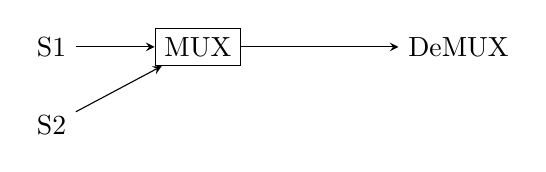
\begin{tikzpicture}[auto, node distance=1cm, >=stealth]
        \node (s1) {S1};
        \node [below=0.5cm of s1] (s2) {S2};
        \node [draw, rectangle, right=1cm of s1] (mux) {MUX};
        \node [right=2cm of mux] (dmux) {DeMUX};
        
        \draw[->] (s1) -- (mux);
        \draw[->] (s2) -- (mux);
        \draw[->] (mux) -- (dmux);
    \end{tikzpicture}
    \captionof{figure}{Basic TDM}
    \end{center}

    \begin{mnemonicbox}
    "TSSBSR" - Time Slots Shared But Sync Required
    \end{mnemonicbox}
\end{solutionbox}

\end{document}
